\chapter{\textit{Designs} do \textit{Figma}}
\label{AppendixC}

O seguinte Apêndice apresenta os \textit{designs} do \textit{mockup}  desenvolvido na plataforma Figma para o projeto em questão. A criação deste protótipo surgiu da ênfase dada à área de \textit{Frontend} durante o estágio, sendo a idealização da interface e a organização da informação elementos fundamentais para um desenvolvimento mais ágil, coerente e orientado.

O objetivo principal do \textit{mockup} foi validar a arquitetura de informação, a experiência do utilizador e a adequação visual da plataforma às necessidades da empresa.

O protótipo serviu como base de referência para a implementação da interface, reduzindo ambiguidades e acelerando o processo de desenvolvimento ao fornecer uma visão clara das funcionalidades e do seu comportamento esperado. Este foi submetido à empresa, que o aprovou e forneceu um \textit{feedback} positivo, validando as decisões de \textit{design} tomadas.

As imagens seguintes ilustram algumas das páginas principais do protótipo, incluindo o painel de controlo, a personalização de métricas e a criação de objetivos.

\begin{figure}[H]
\centering
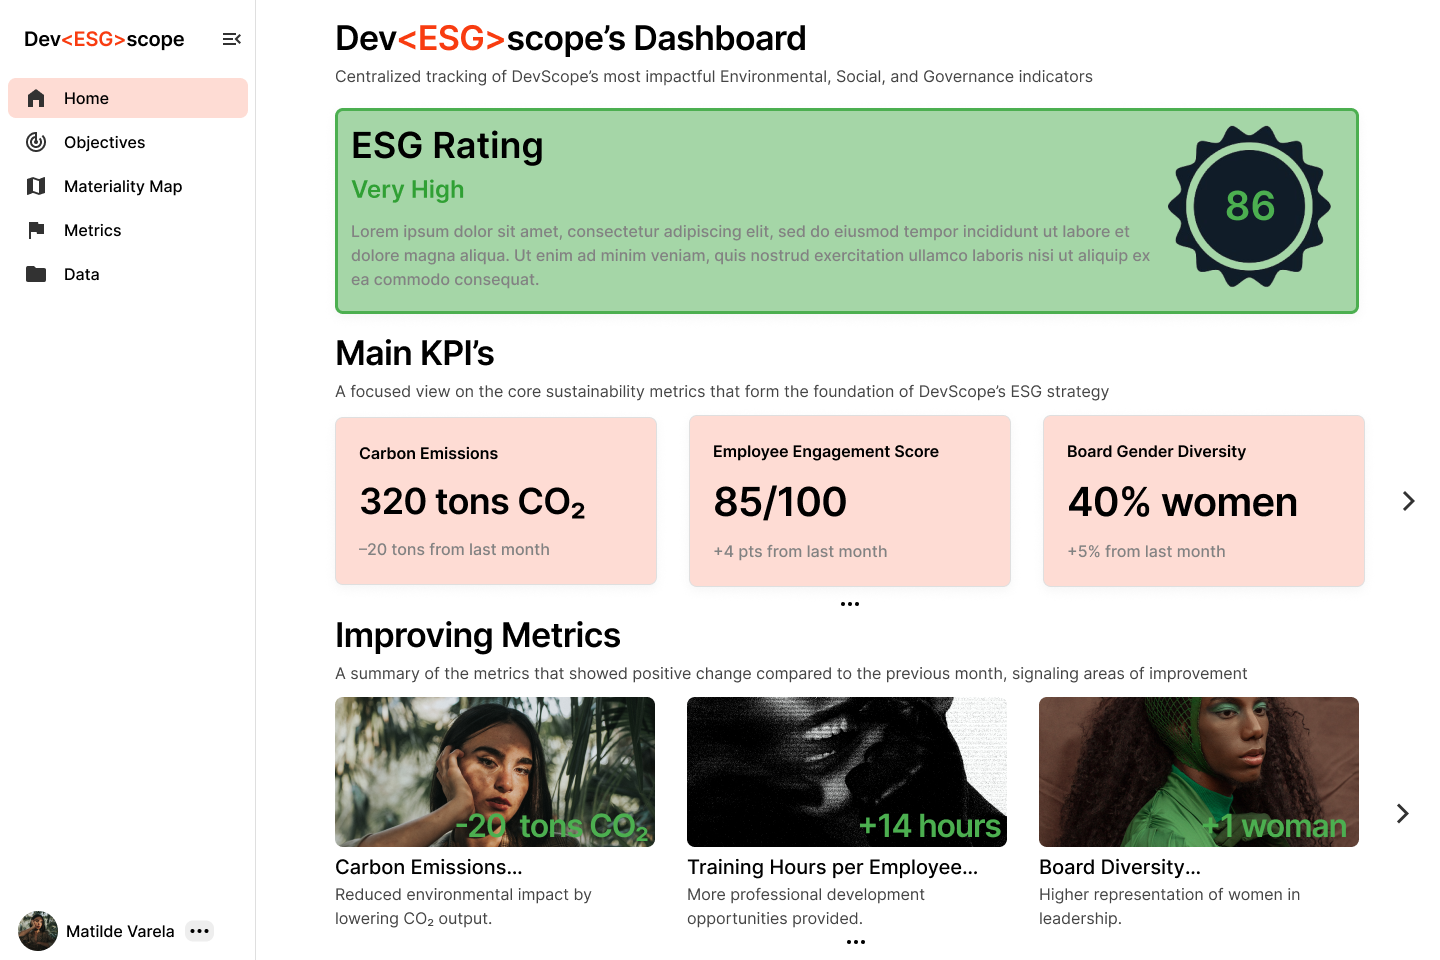
\includegraphics[width=\linewidth]{/frontmatter/assets/mockup/Dashboard _ Home Page.png}
\captionof{figure}{Página Inicial (Dashboard) da Plataforma ESG (autoria própria)}
    \label{fig:dashboardESG}
\end{figure}

%-----------------------------------------------------------

\begin{landscape}
\centering
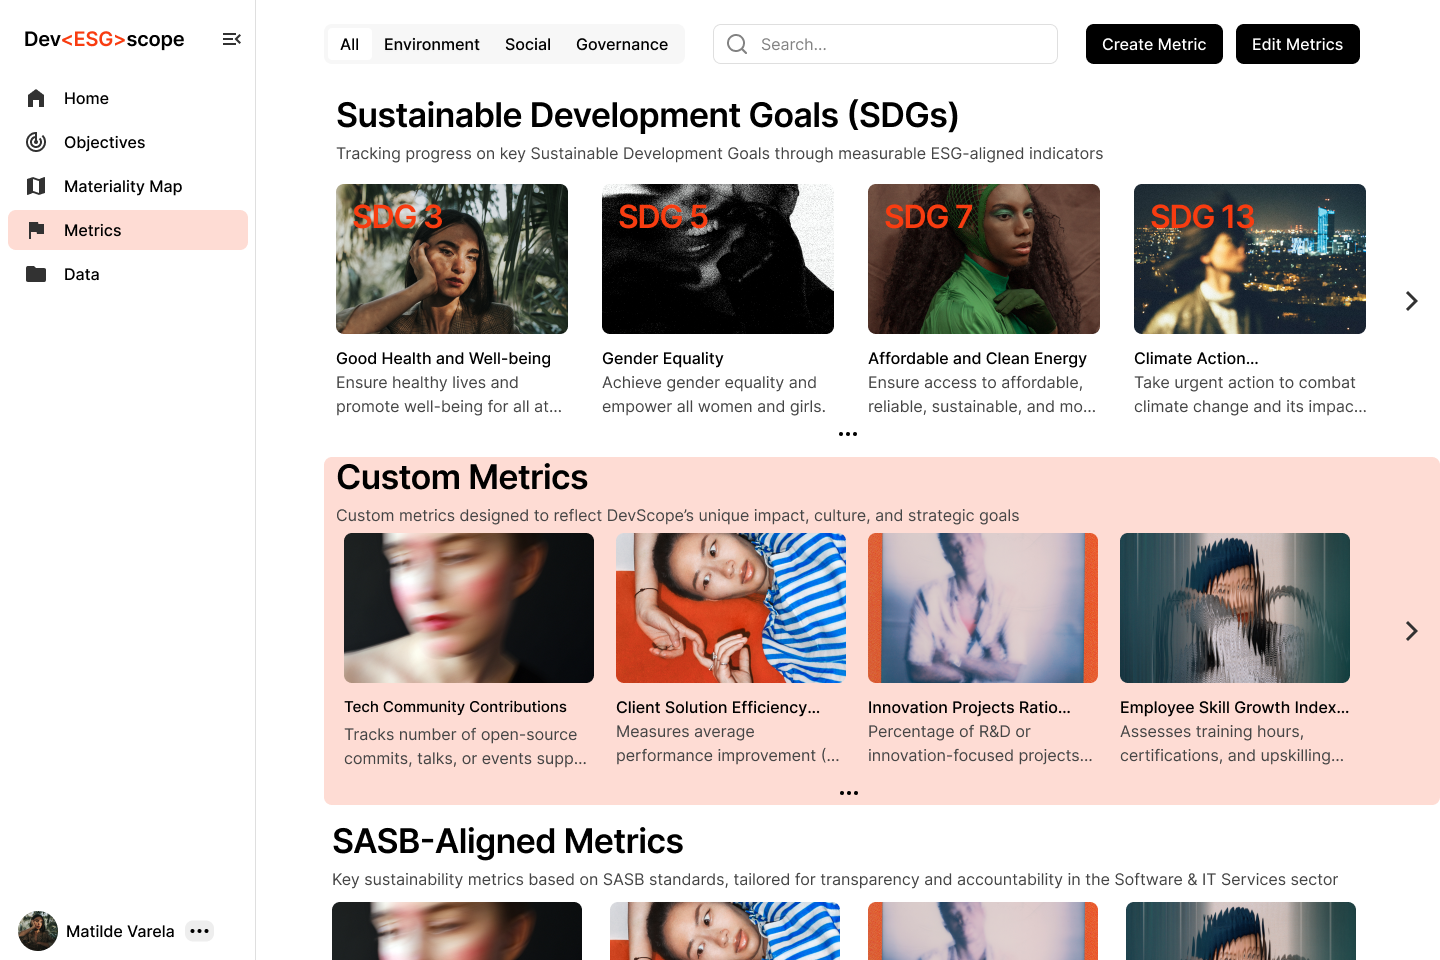
\includegraphics[width=0.9\linewidth]{frontmatter/assets/mockup/Metrics_and_ODS_Customization.png}
\captionof{figure}{Página das Métricas Customizáveis e de SASB (autoria própria)}
\label{fig:metricPage}
\end{landscape}


\begin{figure}[H]
    \centering
    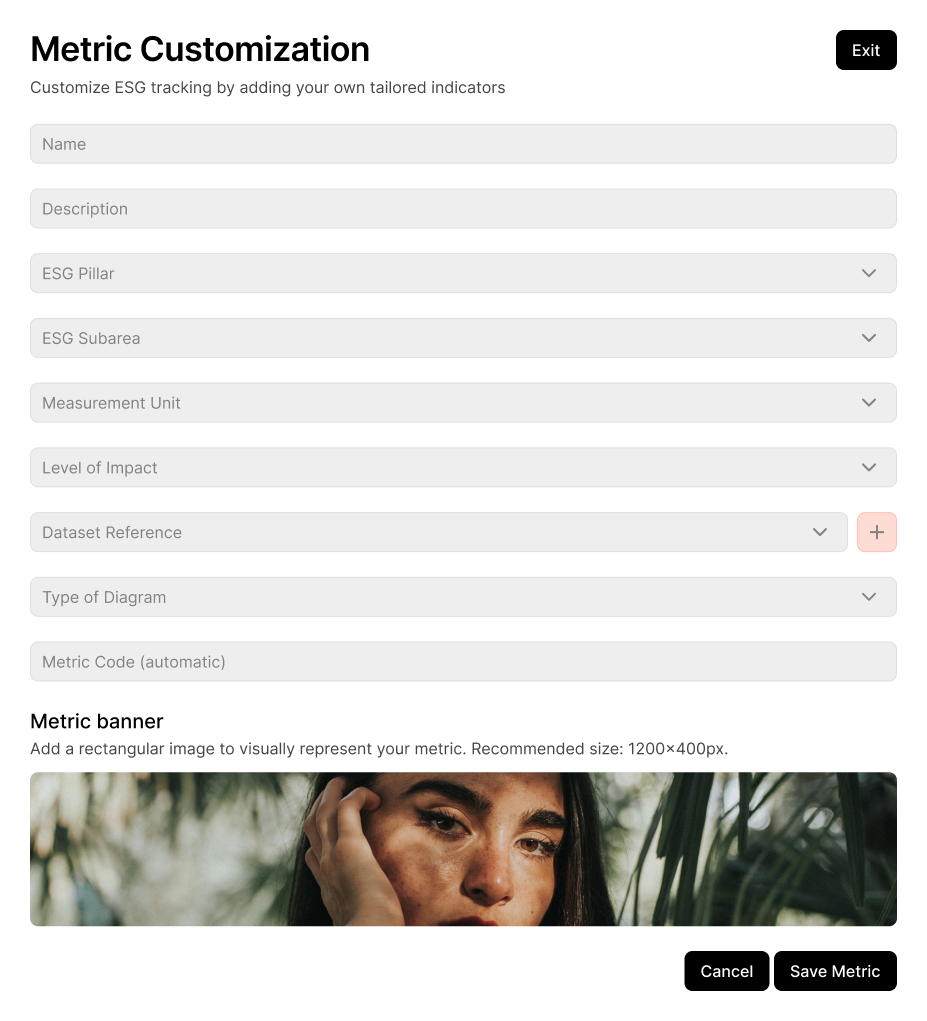
\includegraphics[width=\linewidth]{frontmatter/assets/mockup/Custom Metric Creation.png}
    \caption{Painel de Criação de Métricas Customizáveis (autoria própria)}
    \label{fig:customMetricModal}
\end{figure}


\begin{figure}[H]
    \centering
    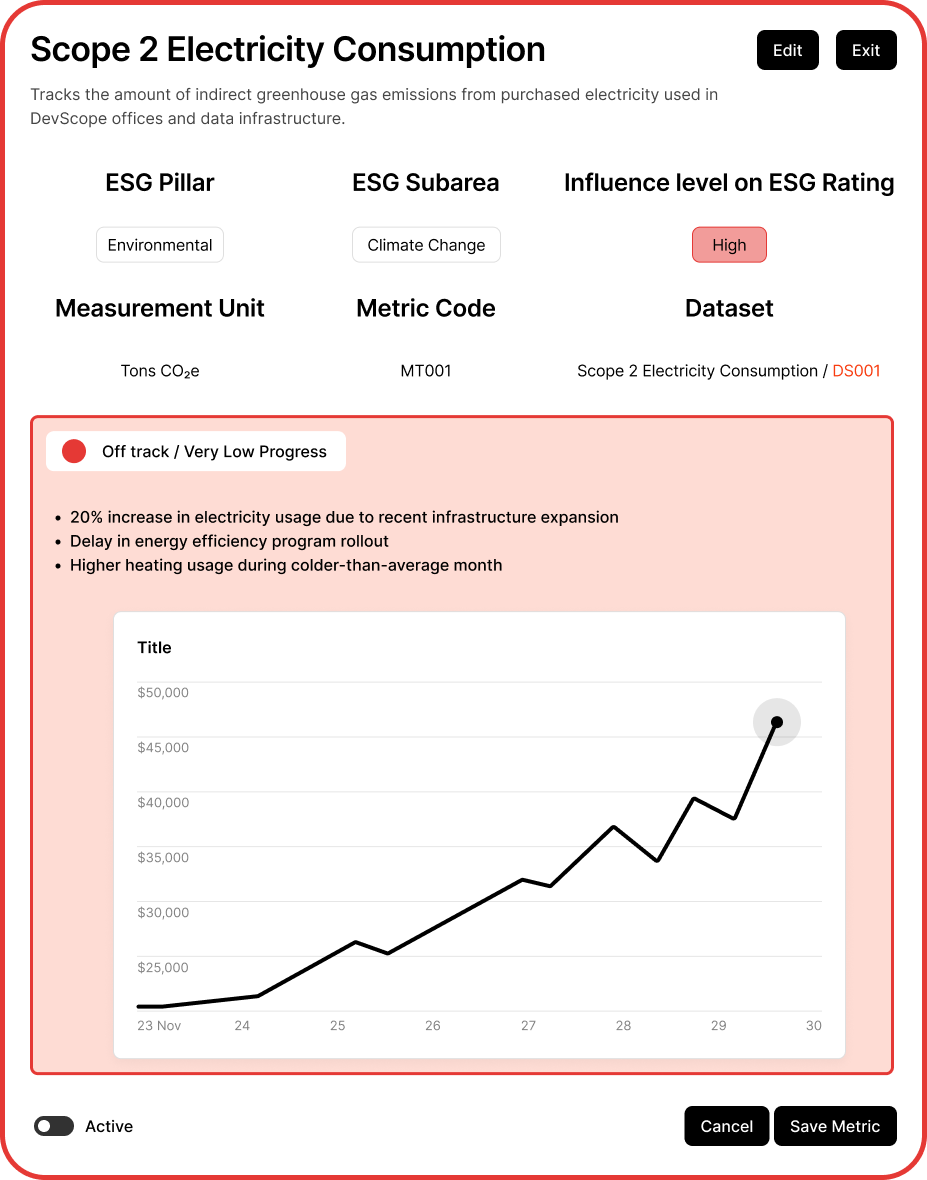
\includegraphics[width=\linewidth]{frontmatter/assets/mockup/Metric Card.png}
    \caption{Painel de Informação da Métrica (autoria própria)}
    \label{fig:metricInfoModal}
\end{figure}

%-----------------------------------------------------------

\begin{figure}[H]
    \centering
    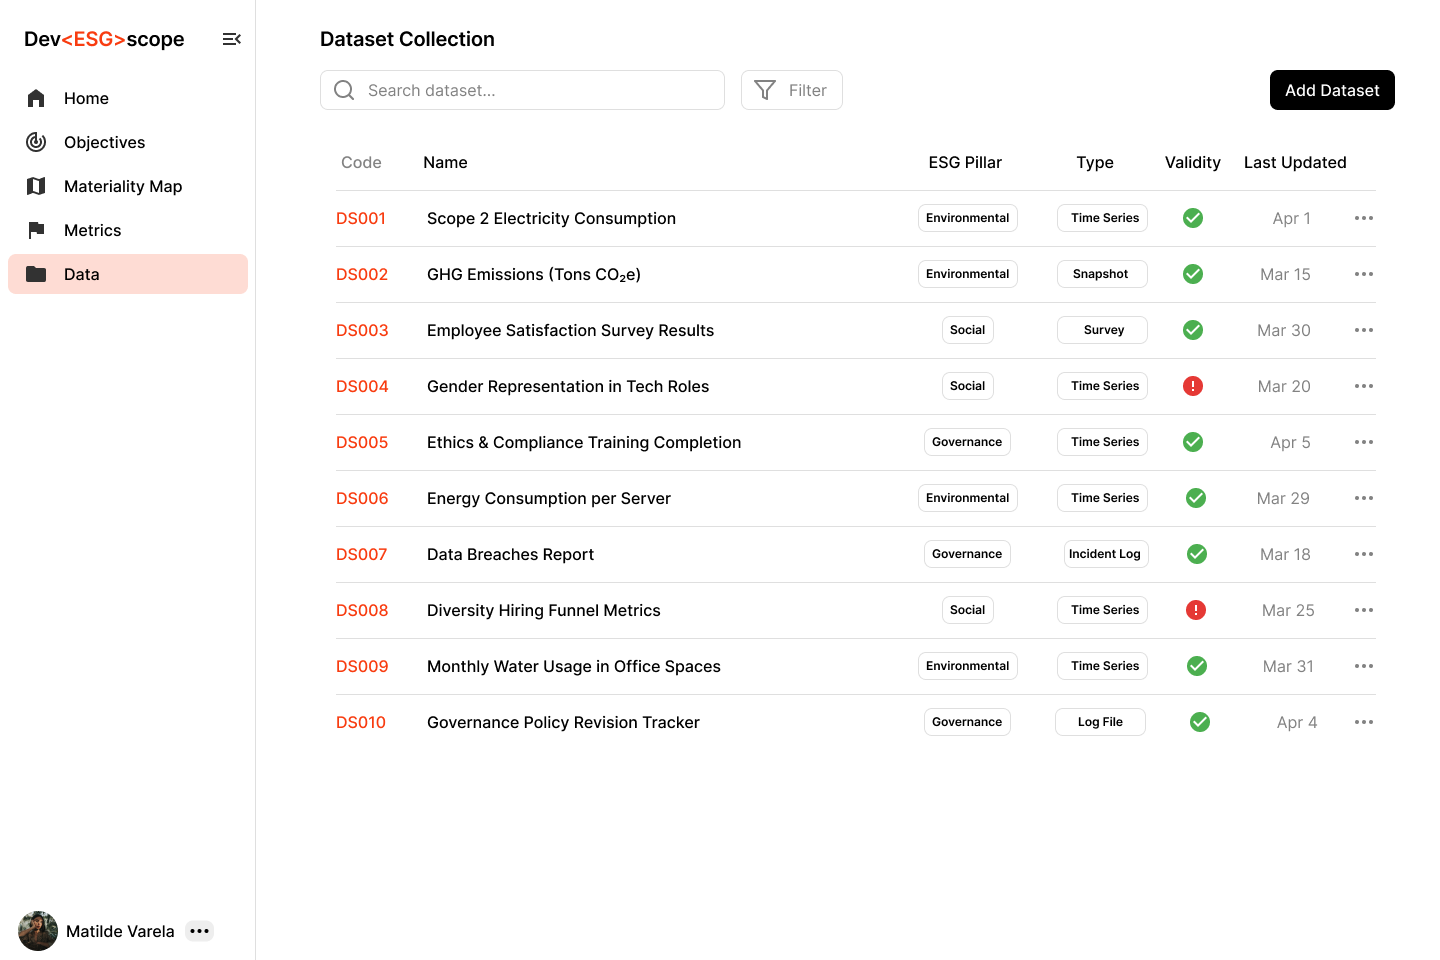
\includegraphics[width=\linewidth]{frontmatter/assets/mockup/Data Collection Database.png}
    \caption{Página dos Conjuntos de Dados (autoria própria)}
    \label{fig:datasetPage}
\end{figure}

\begin{figure}[H]
    \centering
    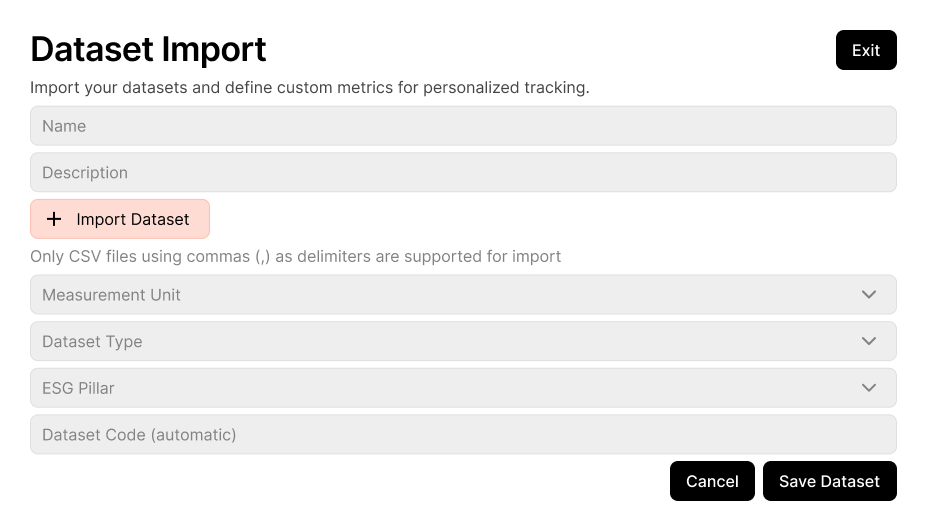
\includegraphics[width=\linewidth]{frontmatter/assets/mockup/Data Import.png}
    \caption{Painel de Importação de Conjuntos de Dados (autoria própria)}
    \label{fig:importDatasetModal}
\end{figure}

%-----------------------------------------------------------

\begin{figure}[H]
    \centering
    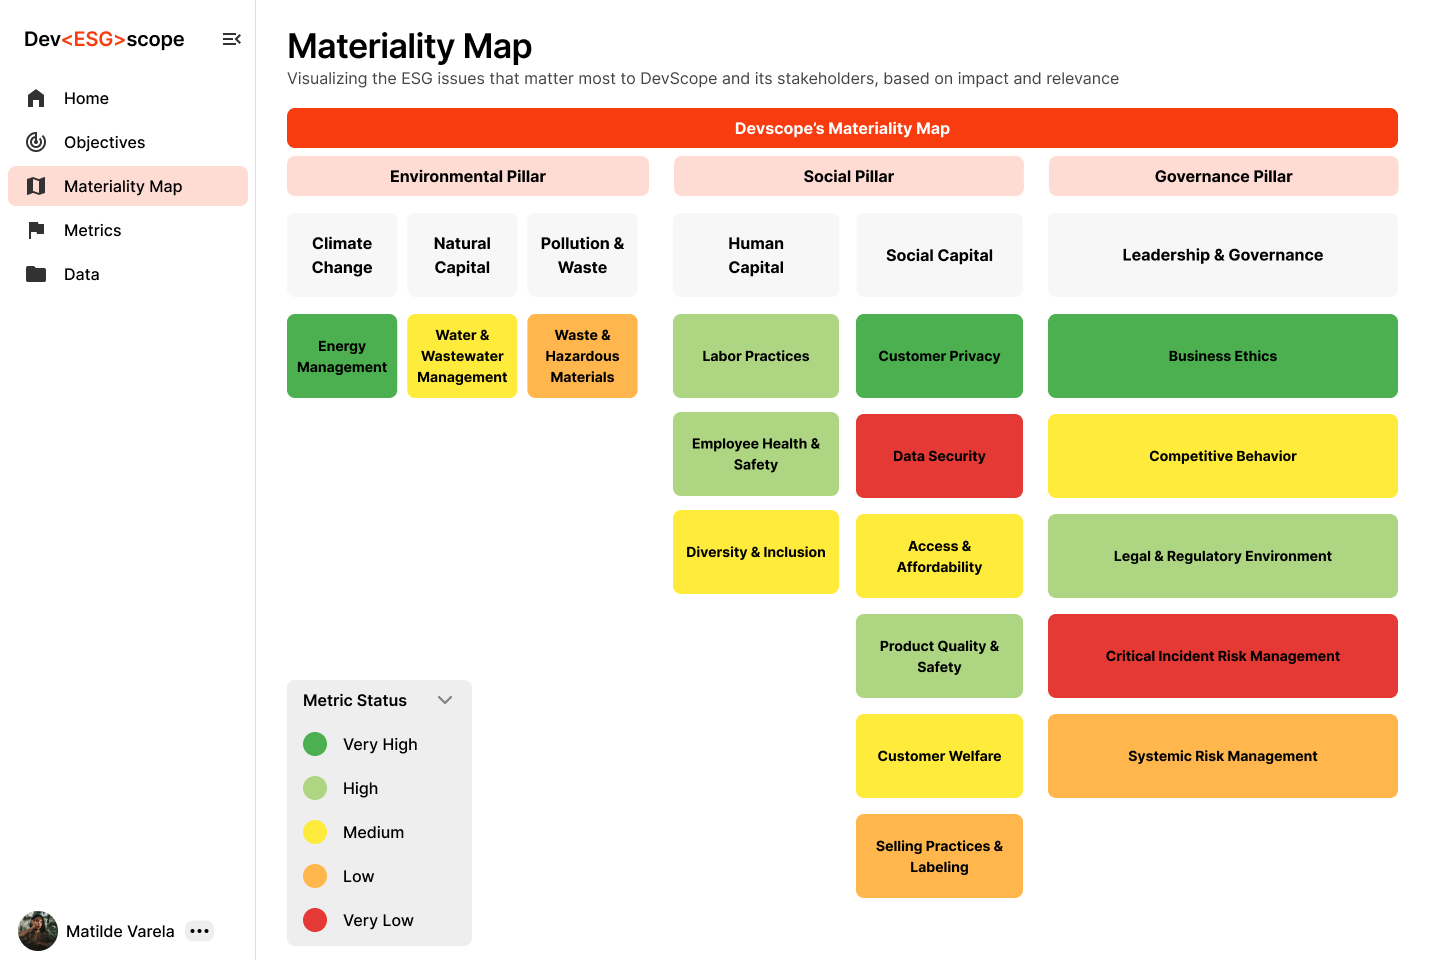
\includegraphics[width=\linewidth]{frontmatter/assets/mockup/Matrix.png}
    \caption{Matriz de Materialidade segundo o setor de \textit{Software} e Serviços IT da \gls{SASB} (autoria própria)}
    \label{fig:matrixPage}
\end{figure}

%-----------------------------------------------------------

\begin{figure}[H]
    \centering
    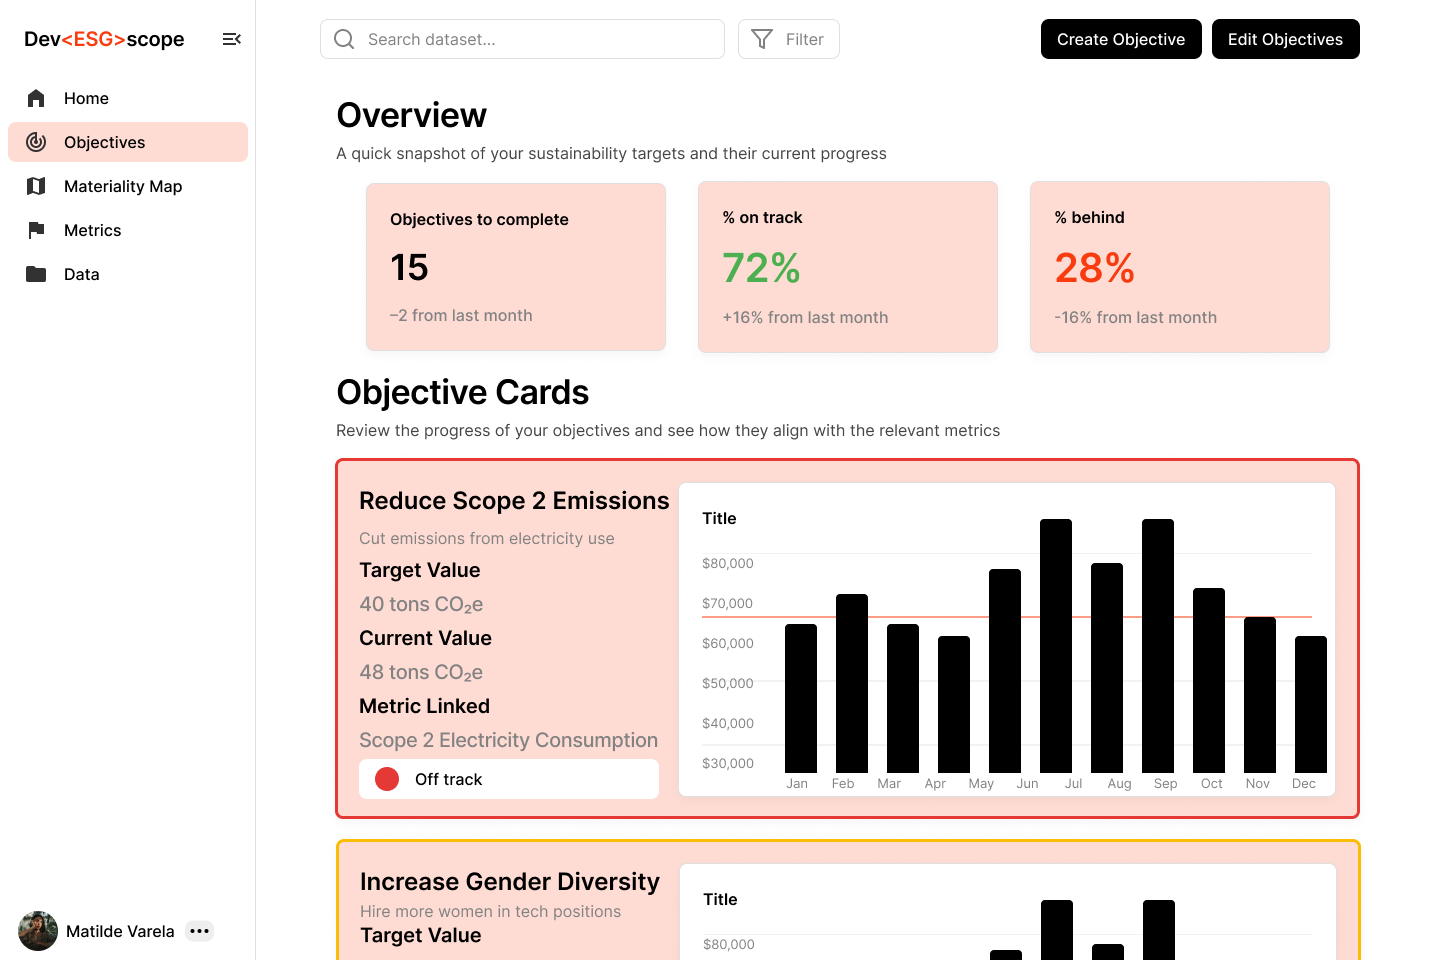
\includegraphics[width=\linewidth]{frontmatter/assets/mockup/Objective Tracking + Comparision with current Metrics.png}
    \caption{Página dos Objetivos (autoria própria)}
    \label{fig:objectivePage}
\end{figure}

\begin{figure}[H]
    \centering
    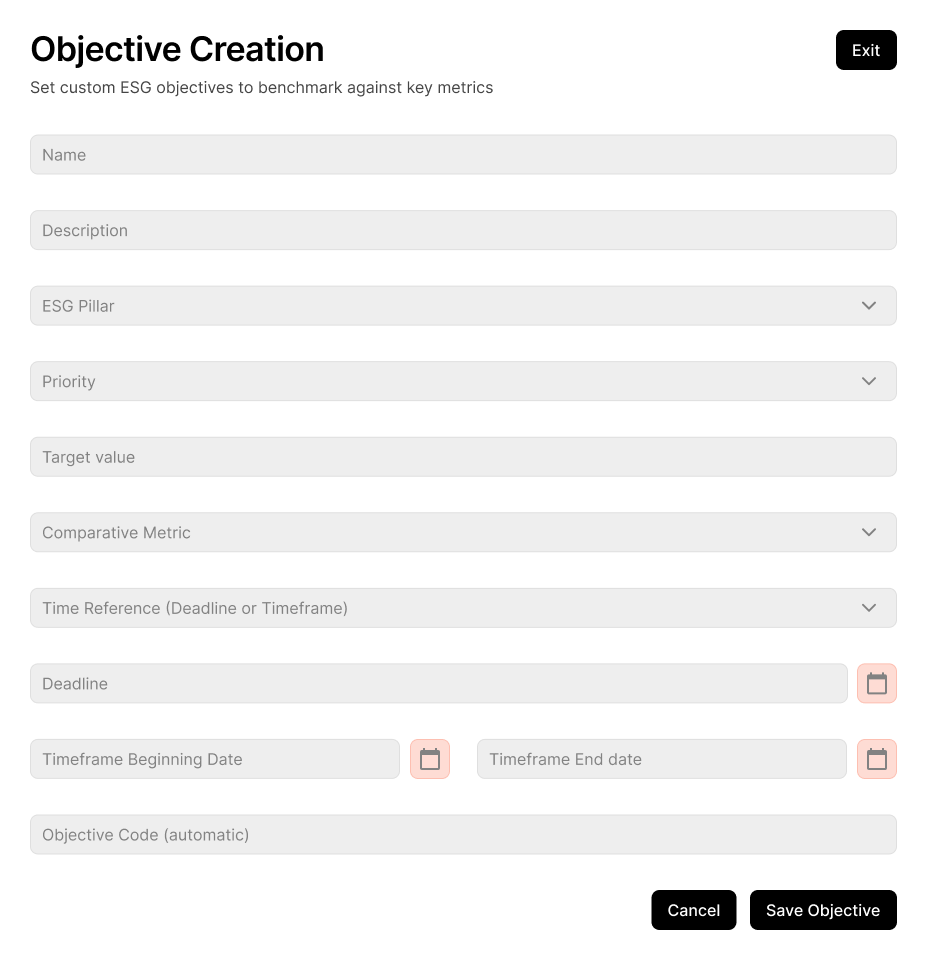
\includegraphics[width=\linewidth]{frontmatter/assets/mockup/Objective Creation.png}
    \caption{Painel de Criação de Objetivos (autoria própria)}
    \label{fig:customObjectiveModal}
\end{figure}